\documentclass{homework}
\usepackage{xcolor}
\usepackage{nicematrix}
\usepackage{booktabs}
\usepackage{enumitem}
\usepackage{caption}
\usepackage{subcaption}
\usepackage{leftidx}
\usepackage{tikz}

\NiceMatrixOptions{cell-space-limits = 1pt}

\title{Solutions Excercise 2}
\author{
  Maksimov, Dmitrii\\
  \texttt{dmitrii.maksimov@fau.de}
  \and
  Ilia, Dudnik\\
  \texttt{ilia.dudnik@fau.de}
}

\tikzset{
  treenode/.style = {shape=rectangle, rounded corners,
                     draw, align=center,
                     top color=white, bottom color=blue!20},
  root/.style     = {treenode, font=\Large, bottom color=green!30},
  env/.style      = {treenode, font=\ttfamily\normalsize},
  NF/.style      = {treenode, font=\ttfamily\normalsize, bottom color=red!30},
  dummy/.style    = {circle,draw}
}

\begin{document}

\maketitle

\exercise
\begin{enumerate}[label=(\alph*)]
\item Consider the subset $M = \{v_1, v_2, v_3, v_4, v_5\} \in \R^5$ with:
\begin{align*}
v_1 &= (1, 0, 0, 0, 0)^T \\
v_2 &= (0, 1, 1, 0, 0)^T \\
v_3 &= (0, 1, 1, 2, 0)^T \\
v_4 &= (0, 0, 0, 0, 1)^T \\
v_5 &= (1, 2, 2, 2, 1)^T
\end{align*}
\begin{enumerate}[label=(\roman*)]
\item the dimension of lin(M)

	The dimension of lin(M) is the maximum number of linearly independent vectors in M:
	\[
	\begin{bNiceArray}{rrrrr}
	        1 & 0 & 0 & 0 & 0 \\
	        0 & 1 & 1 & 0 & 0 \\
	        0 & 1 & 1 & 2 & 0 \\
		0 & 0 & 0 & 0 & 1 \\
		1 & 2 & 2 & 2 & 1 \\
	\end{bNiceArray}
	\Rightarrow
	\begin{bNiceArray}{rrrrr}
	        1 & 0 & 0 & 0 & 0 \\
	        0 & 1 & 1 & 0 & 0 \\
	        0 & 0 & 0 & 2 & 0 \\
		0 & 0 & 0 & 0 & 1 \\
		0 & 0 & 0 & 0 & 0 \\
	\end{bNiceArray}
	\Rightarrow dim(lin(M)) = 4
	\]
\item the affine rank of M

affrang(M) is the cardinality of the largest affinely independent subset of M:
	\[
	\begin{bNiceArray}{rrrrr}
	        -1 & 1 & 1 & 0 & 0 \\
	        -1 & 1 & 1 & 2 & 0 \\
	        -1 & 0 & 0 & 0 & 0 \\
		0 & 2 & 2 & 2 & 1 \\
	\end{bNiceArray}
	\Rightarrow
	\begin{bNiceArray}{rrrrr}
	        1 & -1 & -1 & 0 & 0 \\
	        0 & 1 & 1 & 0 & 0 \\
	        0 & 0 & 0 & 2 & 0 \\
		0 & 0 & 0 & 0 & 1 \\
	\end{bNiceArray}
	\Rightarrow affrang(M) = 4
	\]
\item the dimension of aff(M)

dim(aff(M)) = affrang(M) = 4
\end{enumerate}
\item From linear independence follows affine independence. Show: The converse does not hold.

Let $v_1 = (2, 0)^T, v_2 = (1, 0), v_3 = (1, 1)$. They are affinely independent, since: $v_2 - v_1$ and $v_3 - v_1$ are linearly independent. However, $v_1 = 2 v_2 \Rightarrow v_1, v_2$ and $v_3$ are affinely independent, but not linearly independent.
\item Show: if $x_1, \dots, x_k, x_k+1 \in \R^n, n \geq k$, are affinely independent, then $x_1 = x_{k+1}, \dots, x_k - x_{k+1}$ are lineraly independent

Consider some $\lambda_1, \dots, \lambda_k$, such that: \[\sum_{i=1}^k \lambda_i(x_i - x_{k+1})=0.\] In accordance with affinely independence: $\sum_{i=1}^{k+1}\lambda_i = 0$. Also, \[\sum_{i=1}^{k+1}\lambda_i x_i = \sum_{i=1}^{k}\lambda_i(x_i - x_{k+1}) + \sum_{i=1}^{k+1}\lambda_i x_{k+1}.\] Hence,  $\sum_{i=1}^{k+1}\lambda_i x_i = 0 \Rightarrow \lambda_i = 0 \forall i$
\end{enumerate}

\exercise
Solve the following optimization problem using branch-and-bound and sketch the branch-andbound tree:
\begin{align*}
	\text{max} \quad
	&4x_1 - x_2 \\
	\text{s.t.} \quad
	&7x_1 - 2x_2 \leq 14 \\
	&x_2 \leq 3 \\
	&2x_1 - 2x_2 \leq 3 \\
	&x_1, x_2 \geq 0 \\
	&x_1, x_2 \in \Z
\end{align*}
For the LP relaxation
\begin{align*}
	\text{max} \quad
	&4x_1 - x_2 \\
	\text{s.t.} \quad
	&7x_1 - 2x_2 \leq 14 \\
	&x_2 \leq 3 \\
	&2x_1 - 2x_2 \leq 3 \\
	&x_1, x_2 \geq 0
\end{align*}
has optimal solution at $(2.9, 3)$ with $Z = 8.4$. Then we consider two cases: $x_1 \geq 3$ and $x_1 \leq 2.$
\begin{enumerate}
	\item $x_1 \geq 3$
	
	The linear programming relaxation
\begin{align*}
	\text{max} \quad
	&4x_1 - x_2 \\
	\text{s.t.} \quad
	&7x_1 - 2x_2 \leq 14 \\
	&x_2 \leq 3 \\
	&2x_1 - 2x_2 \leq 3 \\
	&x_2 \geq 0 \\
	&x_1 \geq 3 \\
\end{align*}
has no feasible solution. Hence, the IP has no feasible solution either.
\item $x_1 \leq 2$

The linear programming relaxation
\begin{align*}
	\text{max} \quad
	&4x_1 - x_2 \\
	\text{s.t.} \quad
	&7x_1 - 2x_2 \leq 14 \\
	&x_2 \leq 3 \\
	&2x_1 - 2x_2 \leq 3 \\
	&x_1 \leq 2 \\
	&x_1, x_2 \geq 0
\end{align*}
has optimal solution at $(2, 0.5)$ with $Z = 7.5$. Then we consider two cases: $x_2 \geq 1$ and $x_2 \leq 0.$
\begin{enumerate}[label*=\arabic*.]
\item $x_2 \geq 1$

The linear programming relaxation
\begin{align*}
	\text{max} \quad
	&4x_1 - x_2 \\
	\text{s.t.} \quad
	&7x_1 - 2x_2 \leq 14 \\
	&x_2 \leq 3 \\
	&2x_1 - 2x_2 \leq 3 \\
	&x_1 \leq 2 \\
	&x_2 \geq 1 \\
	&x_1 \geq 0
\end{align*}
has optimal solution at $(2, 1)$ with $Z = 7.0$. This is the optimal solution of the IP as well. Currently, the
best value of Z for the original IP is Z = 7.
\item $x_2 \leq 0$

The linear programming relaxation
\begin{align*}
	\text{max} \quad
	&4x_1 - x_2 \\
	\text{s.t.} \quad
	&7x_1 - 2x_2 \leq 14 \\
	&x_2 \leq 0 \\
	&2x_1 - 2x_2 \leq 3 \\
	&x_1 \leq 2 \\
	&x_1, x_2 \geq 0
\end{align*}
has optimal solution at $(1.5, 0)$ with $Z = 6$. Then we consider two cases: $x_1 \geq 2$ and $x_1 \leq 1.$
\begin{enumerate}[label*=\arabic*.]
\item $x_1 \geq 2$

The linear programming relaxation
\begin{align*}
	\text{max} \quad
	&4x_1 - x_2 \\
	\text{s.t.} \quad
	&7x_1 - 2x_2 \leq 14 \\
	&x_2 \leq 0 \\
	&2x_1 - 2x_2 \leq 3 \\
	&x_1 \leq 2 \\
	&x_2 \geq 0 \\
	&x_1 \geq 2
\end{align*}
has no feasible solution. Hence, the IP has no feasible solution either.
\item $x_1 \leq 1$

The linear programming relaxation
\begin{align*}
	\text{max} \quad
	&4x_1 - x_2 \\
	\text{s.t.} \quad
	&7x_1 - 2x_2 \leq 14 \\
	&x_2 \leq 0 \\
	&2x_1 - 2x_2 \leq 3 \\
	&x_1 \leq 1 \\
	&x_1, x_2 \geq 0
\end{align*}
has optimal solution at $(1, 0)$ with $Z = 4.0$. This is the optimal solution of the IP as well. Currently, the
best value of Z for the original IP is Z = 7.
\end{enumerate}
\end{enumerate}
\end{enumerate}
\begin{center}
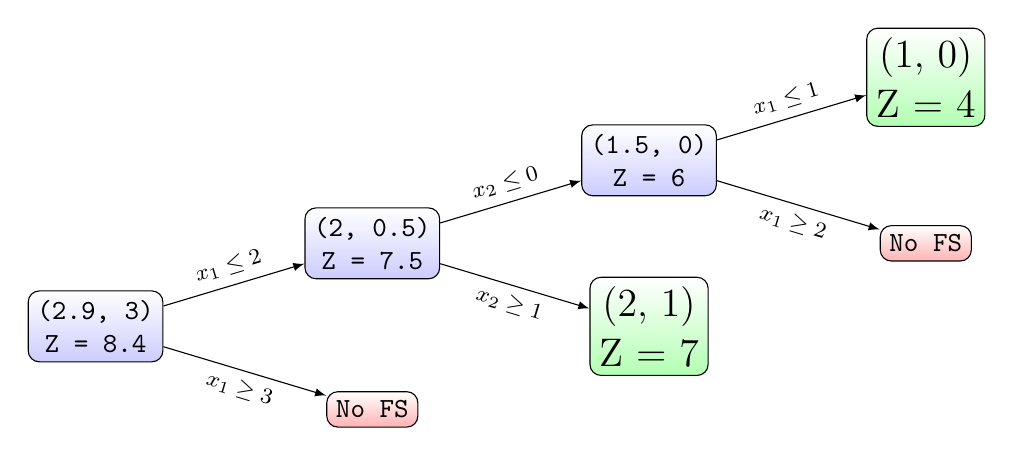
\begin{tikzpicture}
  [
    grow                    = right,
    sibling distance        = 6em,
    level distance          = 10em,
    edge from parent/.style = {draw, -latex},
    every node/.style       = {font=\footnotesize},
    sloped
  ]
  \node [env] {(2.9, 3)\\Z = 8.4}
    child { node [NF] {No FS}
      edge from parent node [below] {$x_1\geq 3$} }
    child { node [env] {(2, 0.5)\\Z = 7.5}
      child { node [root] {(2, 1)\\Z = 7}
        edge from parent node [below] {$x_2\geq1$} }
      child { node [env] {(1.5, 0)\\Z = 6}
	child {node [NF] {No FS}
		edge from parent node [below] {$x_1 \geq 2$}}
	child { node [root] {(1, 0)\\Z = 4}
		edge from parent node [above] {$x_1\leq1$}}
	edge from parent node [above] {$x_2\leq0$}}
              edge from parent node [above] {$x_1\leq2$} };
\end{tikzpicture}
\end{center}
Therefore, the solution (2, 1) with Z = 7 is the optimal solution.
\exercise
Solve the following optimization problem using the simplex algorithm.

\begin{align*}
	\text{max} \quad
	&3x_1 + 2x_2 +4x_3 \\
	\text{s.t.} \quad
	&x_1 + x_2 + 2x_3\leq 4 \\
	&2x_1 + 3x_2 \leq 5 \\
	&x_1, x_2, x_3 \geq 0
\end{align*}
Let slack variables $(s_1, s_2)$ be introduced in each of the restrictions of $\leq$ type, to convert them into equalities, resulting the system of linear equations:
\begin{align*}
  x_1 + x_2 + 2x_3 + s_1 &= 4\\
  2x_1 + 3x_2 + s_2 &= 5.
\end{align*}
Matching the objective function to zero: \[z - 3x_1 - 2x_2 - 4x_3 - 0s_1 - 0s_2 = 0\]
Simplex tableau method:
\begin{equation*}
  \begin{array}{rrrrrr|r}
        &  x_1 &  x_2 &  x_3 & s_1 & s_2 &       \\ \hline
  s_1 & 1     & 1     & 2^\star&   1    &      0 &   4 \\
  s_2 &  2    & 3     &  0    &    0   &      1 &   5 \\ \hline
  z    & -3    & -2    & -4    &    0   &      0 &   0 \\ \hline\hline
  x_3 & \frac{1}{2} &  \frac{1}{2} &  1 &  \frac{1}{2} & \frac{1}{2} & 2\\
  s_2 &  2^\star &  3 &  0 &    0 &   1 &    5 \\ \hline
  z    &  -1 &    0 & 0 &    2 &   0 &   8 \\ \hline\hline
  x_3 & 0 &  \frac{1}{2} &  -\frac{1}{4} &  1 & \frac{1}{2} & \frac{3}{4}\\
  x_1 &  1 &  \frac{3}{2} &  0 &    0 &   \frac{1}{2} & \frac{5}{2} \\ \hline
  z    &  0 &   \frac{3}{2} & 0 &    2 &   0 &   \frac{21}{2}
  \end{array}
\end{equation*}
Hence, $(2.5, 0, 0.75)$ with $z = 10.5$ is the optimal solution.
\end{document}